% CHAPITRE 3
\chapter{Bilan de C de la tourbière de La Guette}
\newpage

\section{Introduction}

\section{Matériels et méthodes}

Distribution des embases aléatoire stratifiée
\subsection{méthodes de mesure}

\subsubsection{mesures de flux de gaz}
La mesure des flux de \coo et de \chh ont été effectué en utilisant la méthode décrite dans la partie~\ref{sec:clsd_chbr_method}.
Les mesures de \coo ont été effectué de mars 2013 à février 2015, avec une fréquence quasiment mensuelle (20 campagnes, pour 24 mois de mesure).

Les mesures de \chh ont été effectuées avec une fréquence moindre principalement liée au difficulté de mise en oeuvre de l'instrument SPIRIT (lourd, difficilement transportable dans un milieu tourbeux).

\subsubsection{Les facteurs contrôlants}

Les mesures manuelle effectuées sont la mesure de la pression atmosphérique, du PAR, des températures du sol à différentes profondeur, de la végétation.

Les mesures automatiquement acquise via une station météo campbell sont la température de l'air, température de la tourbe à X, X et X profondeur, vitesse et direction du vent, humidité relative de l'air, irradiation solaire, pression atmosphérique.

\subsection{modélisation du bilan de C}

Afin de pouvoir interpoler les mesures de respiration mensuelles, il est nécessaire de les relier à des variables environnementales nous l'avons vu.
Un des facteurs de contrôle des flux est la température qui régule les processus chimiques et biologiques.
La température à \SI{-5}{\cm} est la plus souvent utilisée \cite{ballantyne2014}, même si d'autres comme la température de l'air ou encore la température du sol à \SI{-10}{\cm} peuvent également l'être \cite{bortoluzzi2006,kim1992}.
Cette profondeur, \SI{-5}{\cm}, est régulièrement utilisée car c'est dans la tourbe, proche de la surface qu'est produit la majorité du \coo.
\textbf{production CO2 ? profils ?}
C'est également à des profondeurs relativement faibles que se situent la majorité des racines \plop qui peuvent contribuer à la respiration du sol \textbf{(de l'écosystème?)} pour 35 à \SI{60}{\percent} \cite{silvola1996a,crow2005}.

\section{Évolution générale des facteurs contrôlants et des flux}

\subsection{Les facteurs contrôlants}

Si on observe un étiage en 2013 avec une baisse d'une vingtaine de centimètres du niveau de la nappe en moyenne, en 2014 aucun étiage n'est observable de façon nette.
La nappe d'eau restant en grande majorité au dessus de \SI{-10}{\cm}.

\begin{figure}
\centering
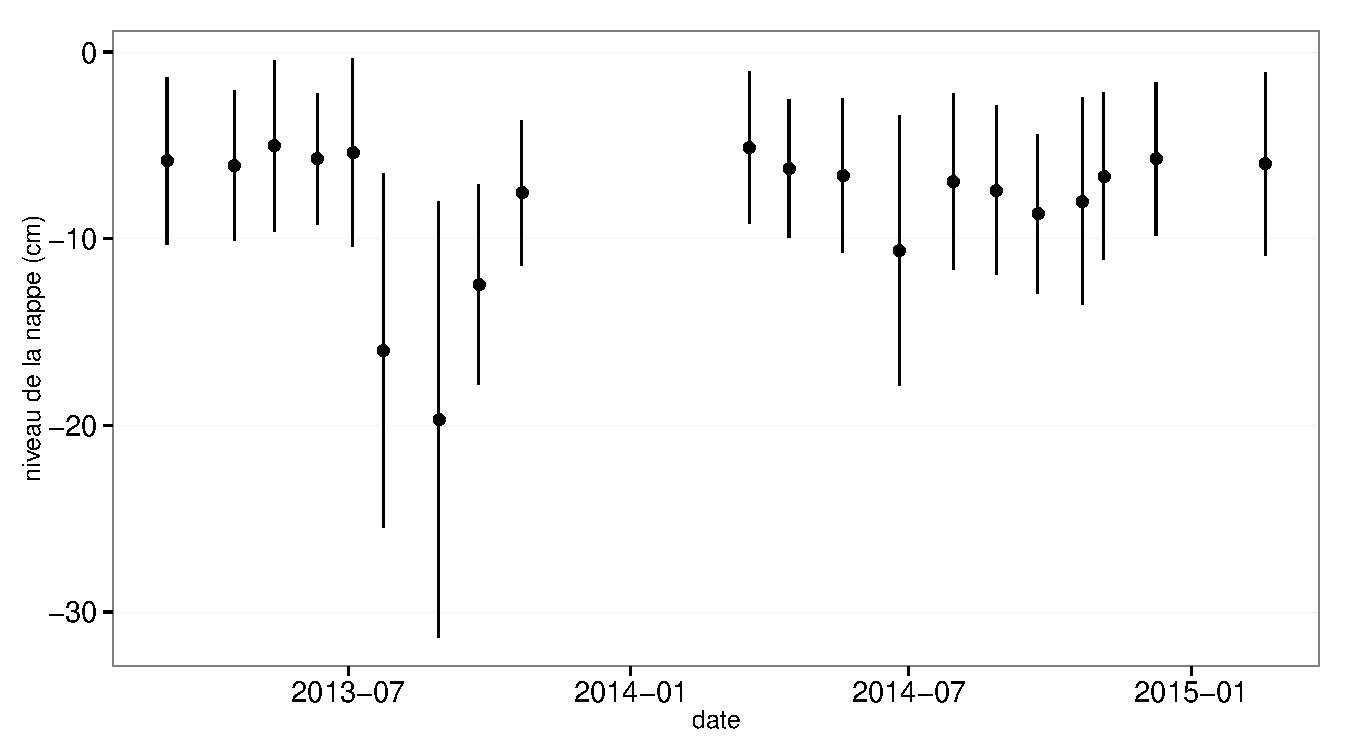
\includegraphics[width=\textwidth]{chap3/WTL_mean_evolution}
\caption{Évolution du niveau de la nappe moyen des 20 embases pendant la période de mesure (mars 2013 -- février 2015)}
\label{fig:WTL_mean_evolution}
\end{figure}

\subsection{Le \coo}

%\subsubsection{PBB}

En moyenne la PPB est de \SI{7.12(519)}{\uml} en 2013 et de \SI{6.56(472)}{\uml} en 2014 (Figure~\ref{fig:GPP_evolution_avg}).
L'amplitude de la PPB est similaire en 2013 et en 2014, avec un maximum autour de \SI{13}{\uml}.


\begin{figure}
	\centering
	\begin{subfigure}[t]{\textwidth}
		\centering
		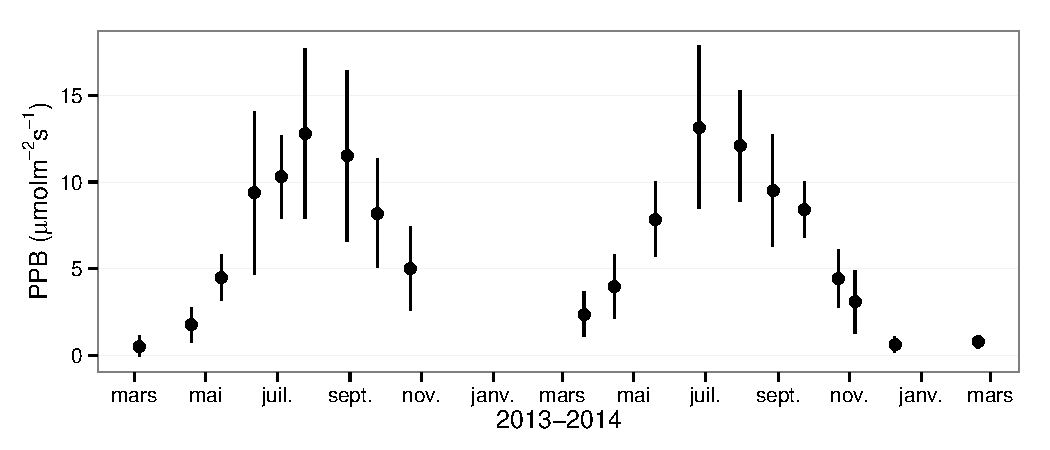
\includegraphics[width=.9\textwidth]{chap3/GPP_evolution_avg}
		\caption{Production primaire brute}
		\label{fig:GPP_evolution_avg}
	\end{subfigure}%
	
	\begin{subfigure}[t]{\textwidth}
		\centering
		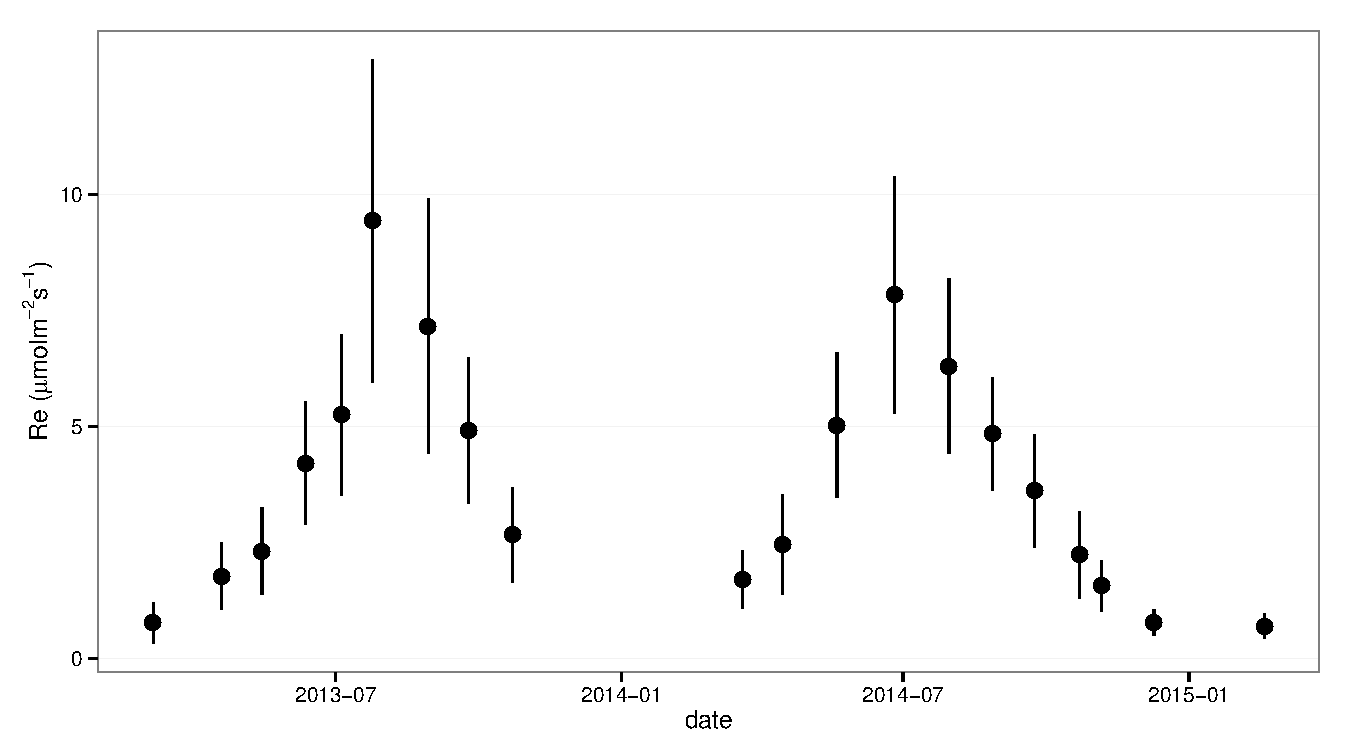
\includegraphics[width=.9\textwidth]{chap3/ER_evolution_avg}
		\caption{Respiration de l'écosystème}
		\label{fig:ER_evolution_avg}
	\end{subfigure}
	
	\begin{subfigure}[t]{\textwidth}
		\centering
		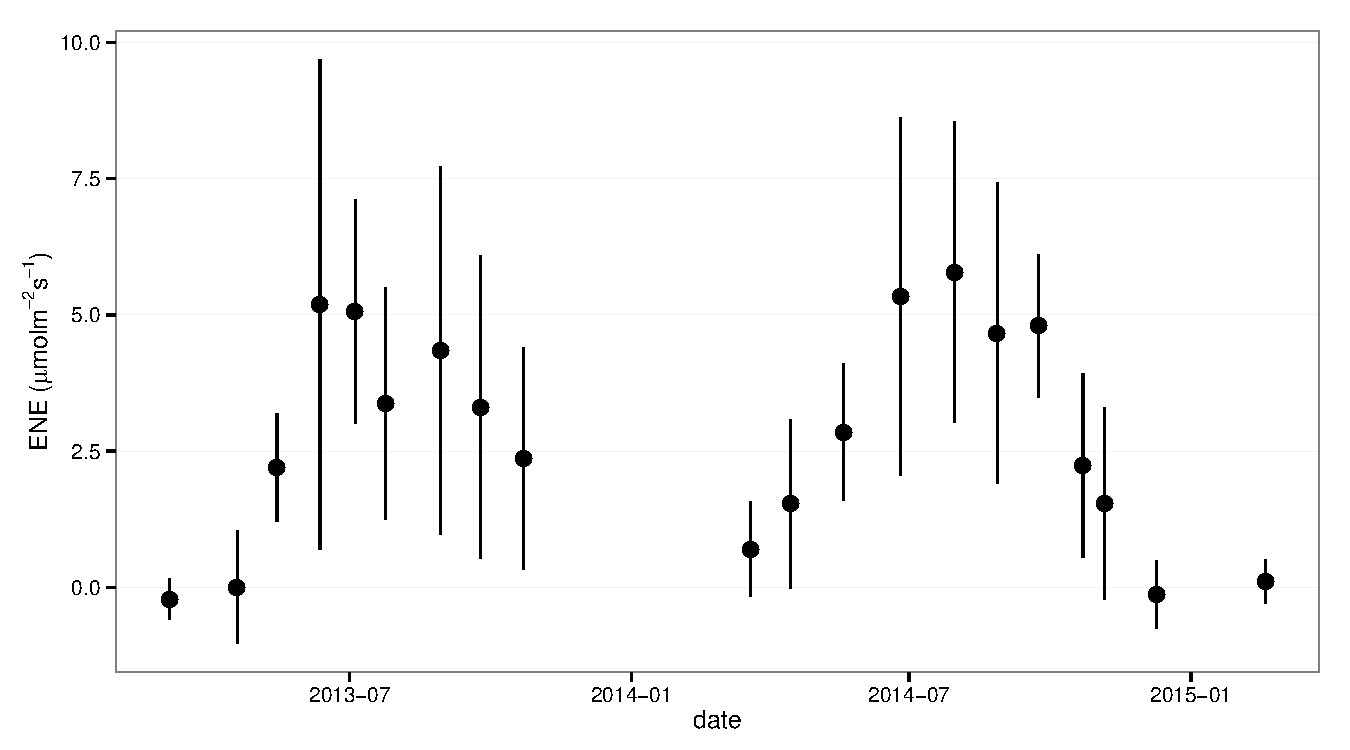
\includegraphics[width=.9\textwidth]{chap3/NEE_evolution_avg}
		\caption{Échange net de l'écosystème}
		\label{fig:NEE_evolution_avg}
	\end{subfigure}
\caption{Évolution du niveau de PPB, RE et ENE pendant la période de mesure. Moyenne des 20 embases de mars 2013 à février 2015.}
\label{fig:flux_evolution_avg}
\end{figure}

%\begin{figure}
%\centering
%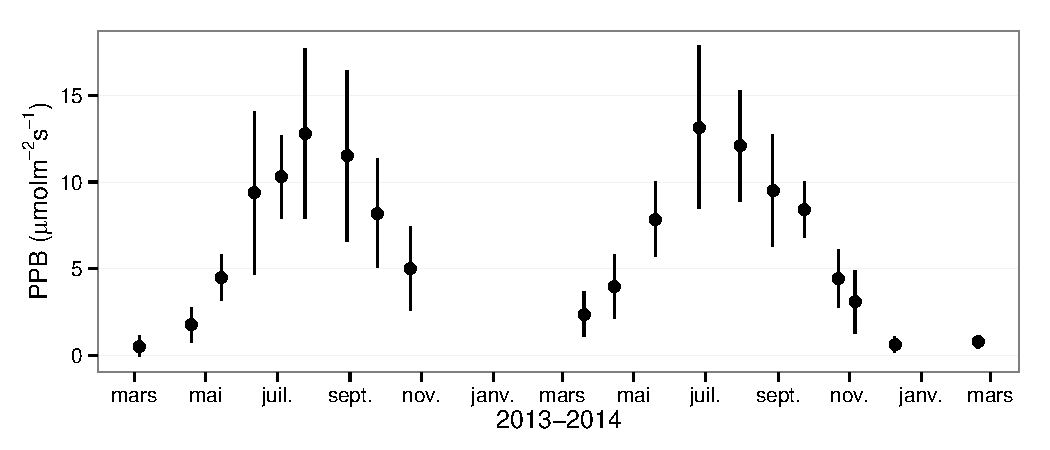
\includegraphics[width=\textwidth]{chap3/GPP_evolution_avg}
%\caption{Évolution du niveau de la production primaire brute, moyenne des 20 embases pendant la période de mesure (mars 2013 -- février 2015)}
%\label{fig:GPP_evolution_avg}
%\end{figure}

%\subsubsection{ER}

La respiration de l'écosystème atteint presque \SI{10}{\uml} en août 2013, tandis qu'elle ne dépasse pas \SI{8}{\uml} en 2014 (Figure~\ref{fig:ER_evolution_avg}).
Les valeurs moyenne de respiration en 2013 et 2014 sont de \SI{4.27(316)}{\uml} et \SI{3.63(256)}{\uml} respectivement.

%\begin{figure}
%\centering
%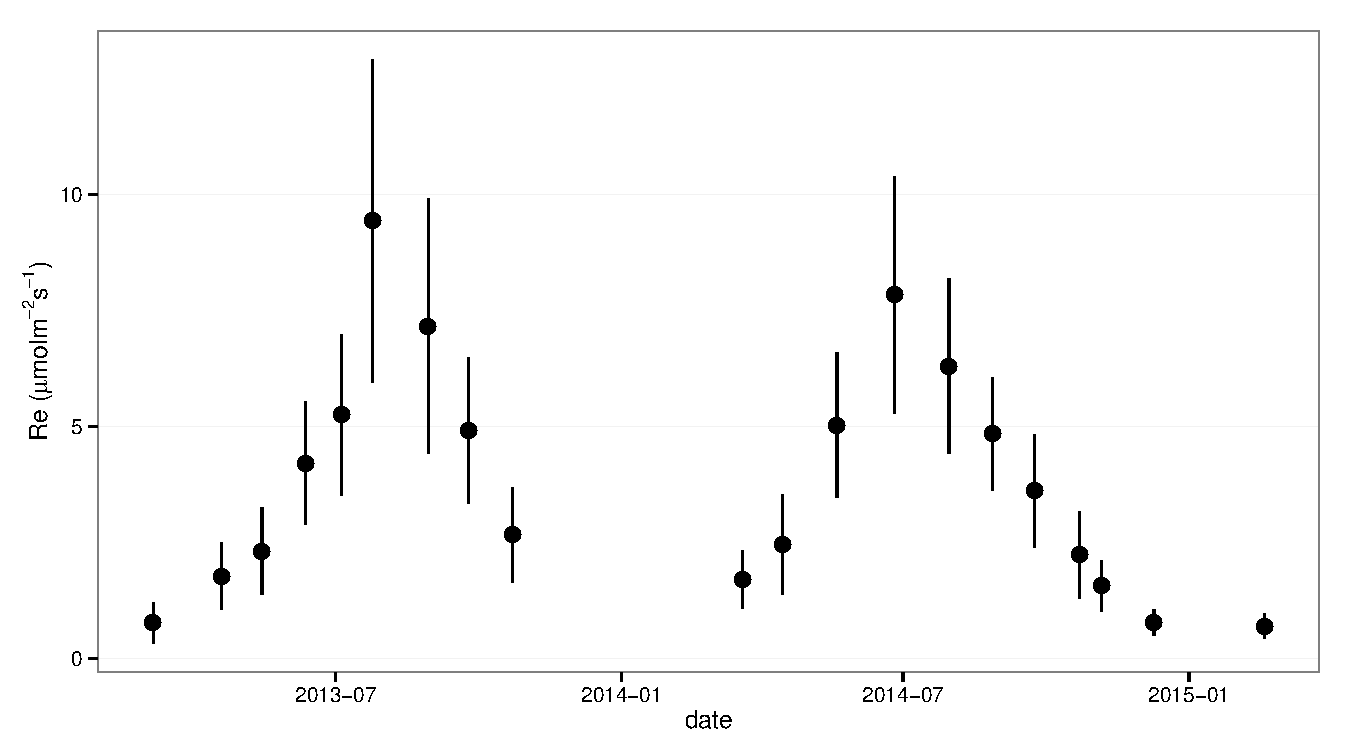
\includegraphics[width=\textwidth]{chap3/ER_evolution_avg}
%\caption{Évolution du niveau de la respiration de l'écosystème, moyenne des 20 embases pendant la période de mesure (mars 2013 -- février 2015)}
%\label{fig:ER_evolution_avg}
%\end{figure}

%\subsubsection{ENE}

L'évolution de l'ENE suit une logique saisonnière (Figure~\ref{fig:NEE_evolution_avg}).
En 2013, le maximum est atteint vers \SI{5}{\uml} en juillet.
En 2014, l'ENE est globalement un peu plus importante et monte jusqu'à \SI{6}{\uml} en août.
En moyenne l'ENE est de \SI{2.85(305)}{\uml} en 2013 et de \SI{2.93(277)}{\uml} en 2014.

%\begin{figure}
%\centering
%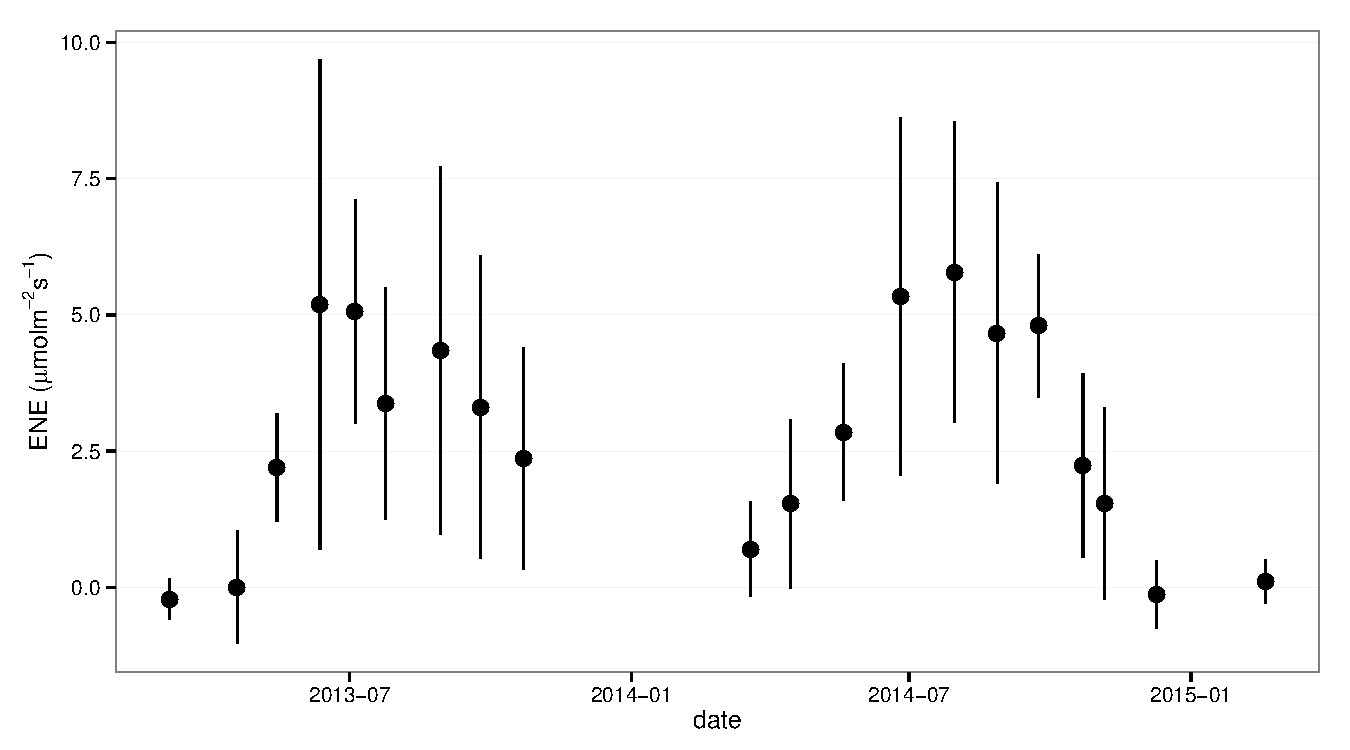
\includegraphics[width=\textwidth]{chap3/NEE_evolution_avg}
%\caption{Évolution du niveau de l'échange net de l'écosystème, moyenne des 20 embases pendant la période de mesure (mars 2013 -- février 2015)}
%\label{fig:NEE_evolution_avg}
%\end{figure}

\subsection{Le \chh}
\subsection{Le Carbone Organique Dissous (COD)}

\section{Le bilan de carbone}

\begin{align}
RE &= a \times exp(b\times T5)\\
PPBsat &= a \times exp(-((Tair - b)/ c)^2)\\
ENE &= PPB - RE\\
ENE &= a \times exp(b\times T5) - a \times exp(-((Tair - b)/ c)^2)
\end{align}
\section{Évaluation du bilan}

\subsection{sensibilité des paramètres}

\subsection{capacité à modéliser d'autres données}

\subsection{représentativité locale}

\section{représentativité locale ?}